
\section{Aspect produits }

\subsection{ Description graphique de la décomposition produit }
	\begin{figure}[H]
	\begin{center}	
		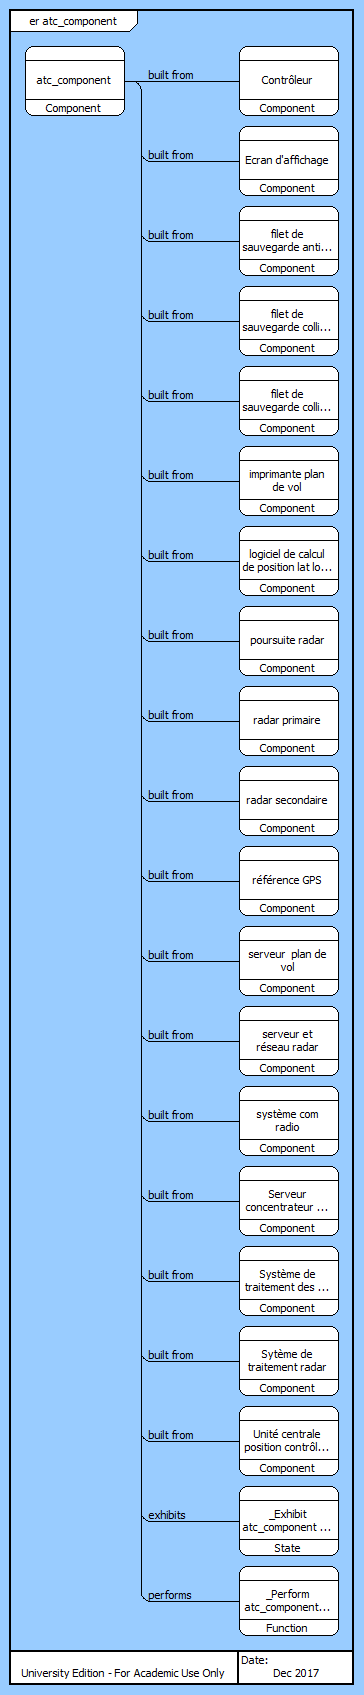
\includegraphics[scale=0.45]{images/atc_component}
		\caption{Diagramme entité-relation des composants du système ATC}
		\label{prod}
	\end{center}
\end{figure}




\begin{landscape}	
	\subsection{ Matrice de traçabilité Fonctions / composants }
	
	
	L'ensemble des fonctions vers l'ensemble des composants doit être une application surjective ; une fonction ne peut être assurée par deux composants différents dans le modèle Vitech core. Par contre, plusieurs composants peuvent effectuer la même fonction. La matrice de la figure \ref{fc} montre une couverture exhaustive des fonctions feuille par les composants du système. En particulier, la contrainte d'affichage unique de l'énoncé est respectée.
	
	\begin{figure}[H]
		\begin{center}	
			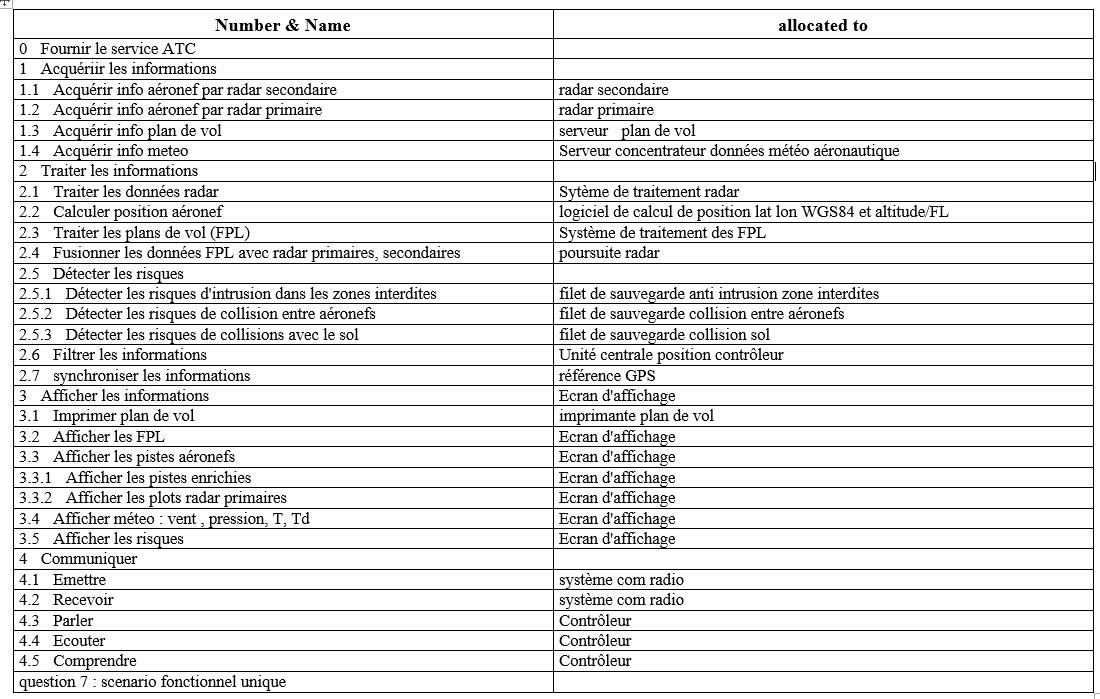
\includegraphics[scale=0.65]{images/trace_fc}
			\caption{Matrice de traçabilité Fonctions / composants }
			\label{fc}
		\end{center}
	\end{figure}	

\end{landscape}


\subsection{ Matrice de traçabilité fonctions/input/output }
La matrice de traçabilité présentée dans les figures \ref{tfio} et \ref{tfio2} s'est avérée essentielle pour vérifier les entrées sorties des fonctions feuille.
En effet, malgré l'utilisation du diagramme N2, des oublis ont persisté ; seules les vues tabulaires permettent l'exhaustivité en mettant en évidence les manques. Ceci facilite l'approche récursive ou itérative propre à tout processus de conception ou développement. 

\paragraph{}
On regrettera le fait que les tables dans CORE ne puissent pas être directement générées au format latex. 

\paragraph{}
Enfin, nous avons noté que le processus itératif se nourrit aussi des divergences potentielles entre l'ensemble des composants et celui des fonctions. On peut ainsi être amené à décomposer une fonction en sous fonctions ou un composant en sous composant. On arrive ainsi à une granularité optimale du FBS et du PBS  par "convergence des deux mondes".  

\begin{landscape}

\begin{figure}[H]
	\begin{center}	
		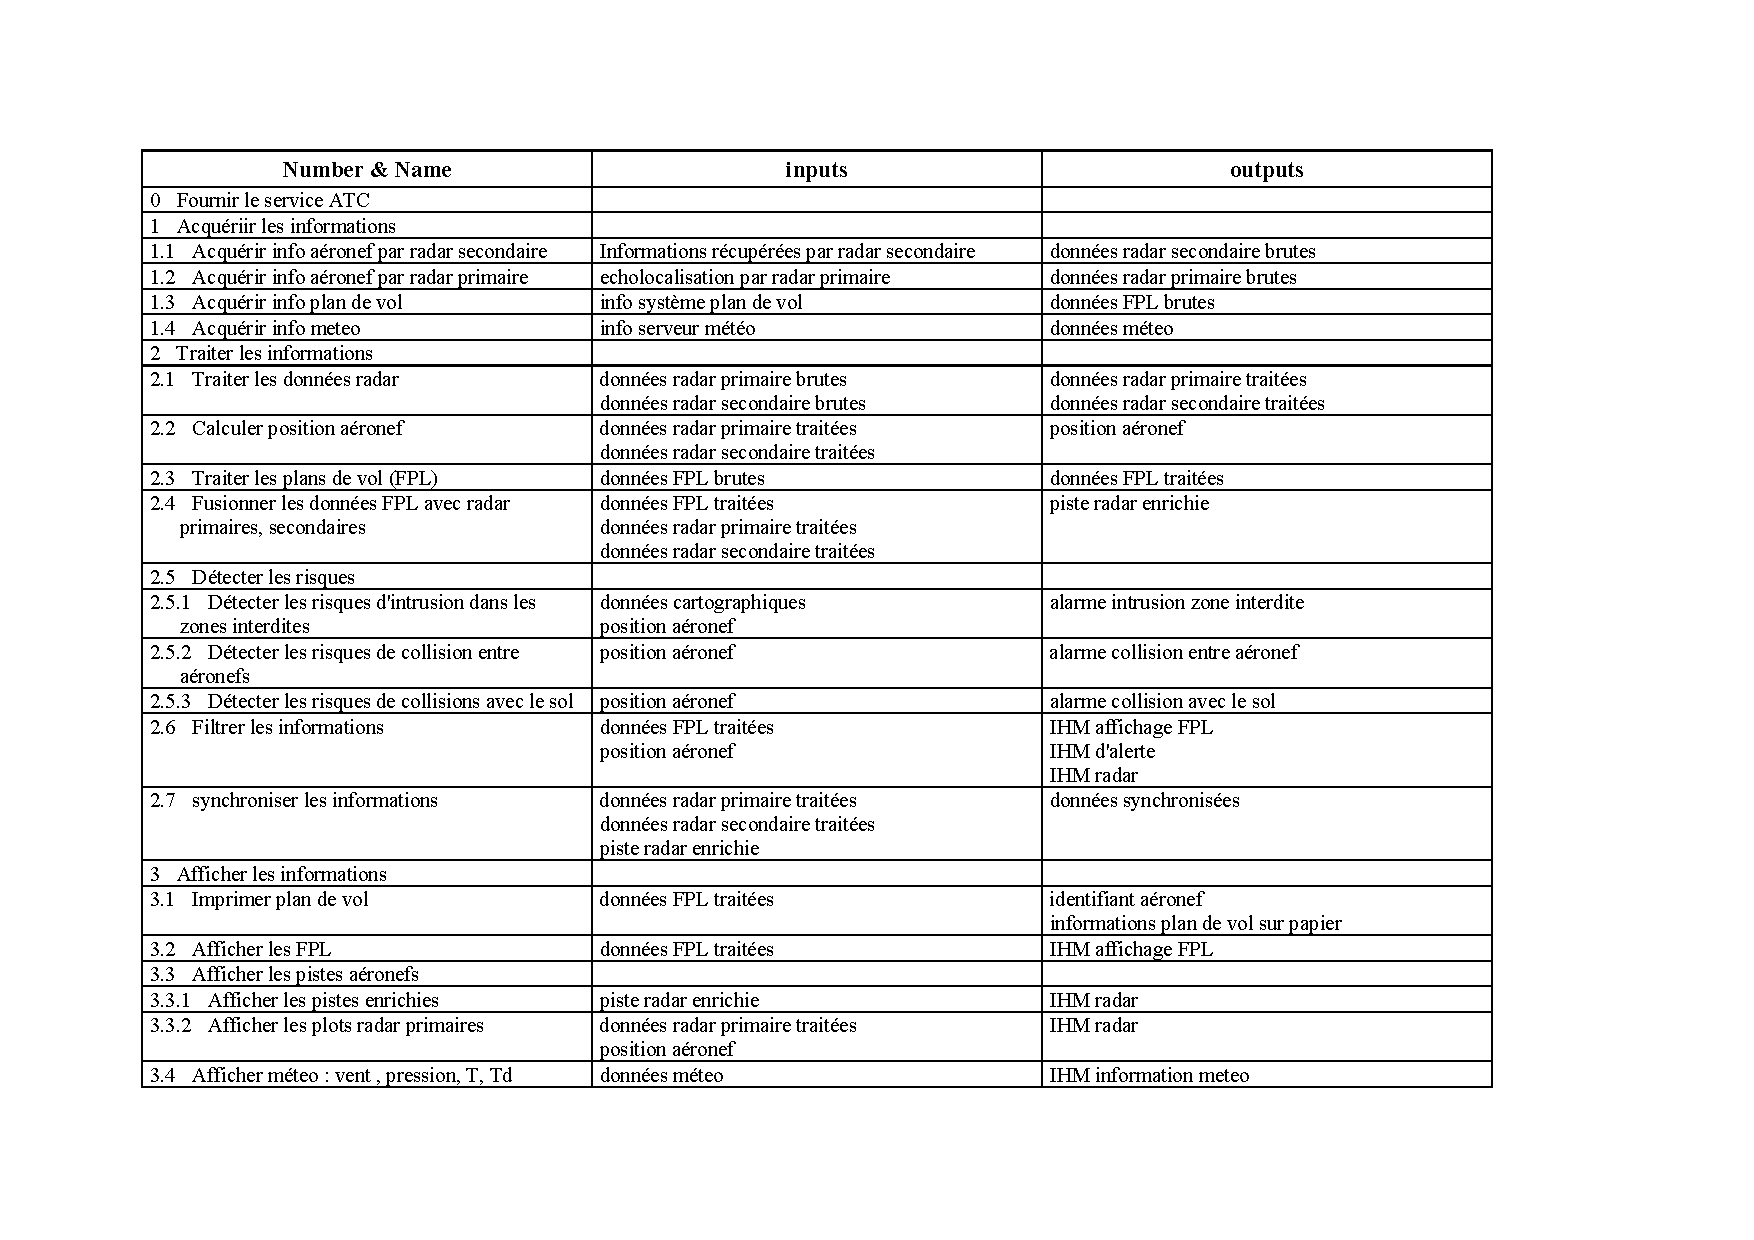
\includegraphics[scale=0.7]{images/tfio}
		
		\caption{Matrice de traçabilité Fonctions / composants }
		\label{tfio}
	\end{center}
\end{figure}
	



	\begin{figure}[H]
		\begin{center}	
			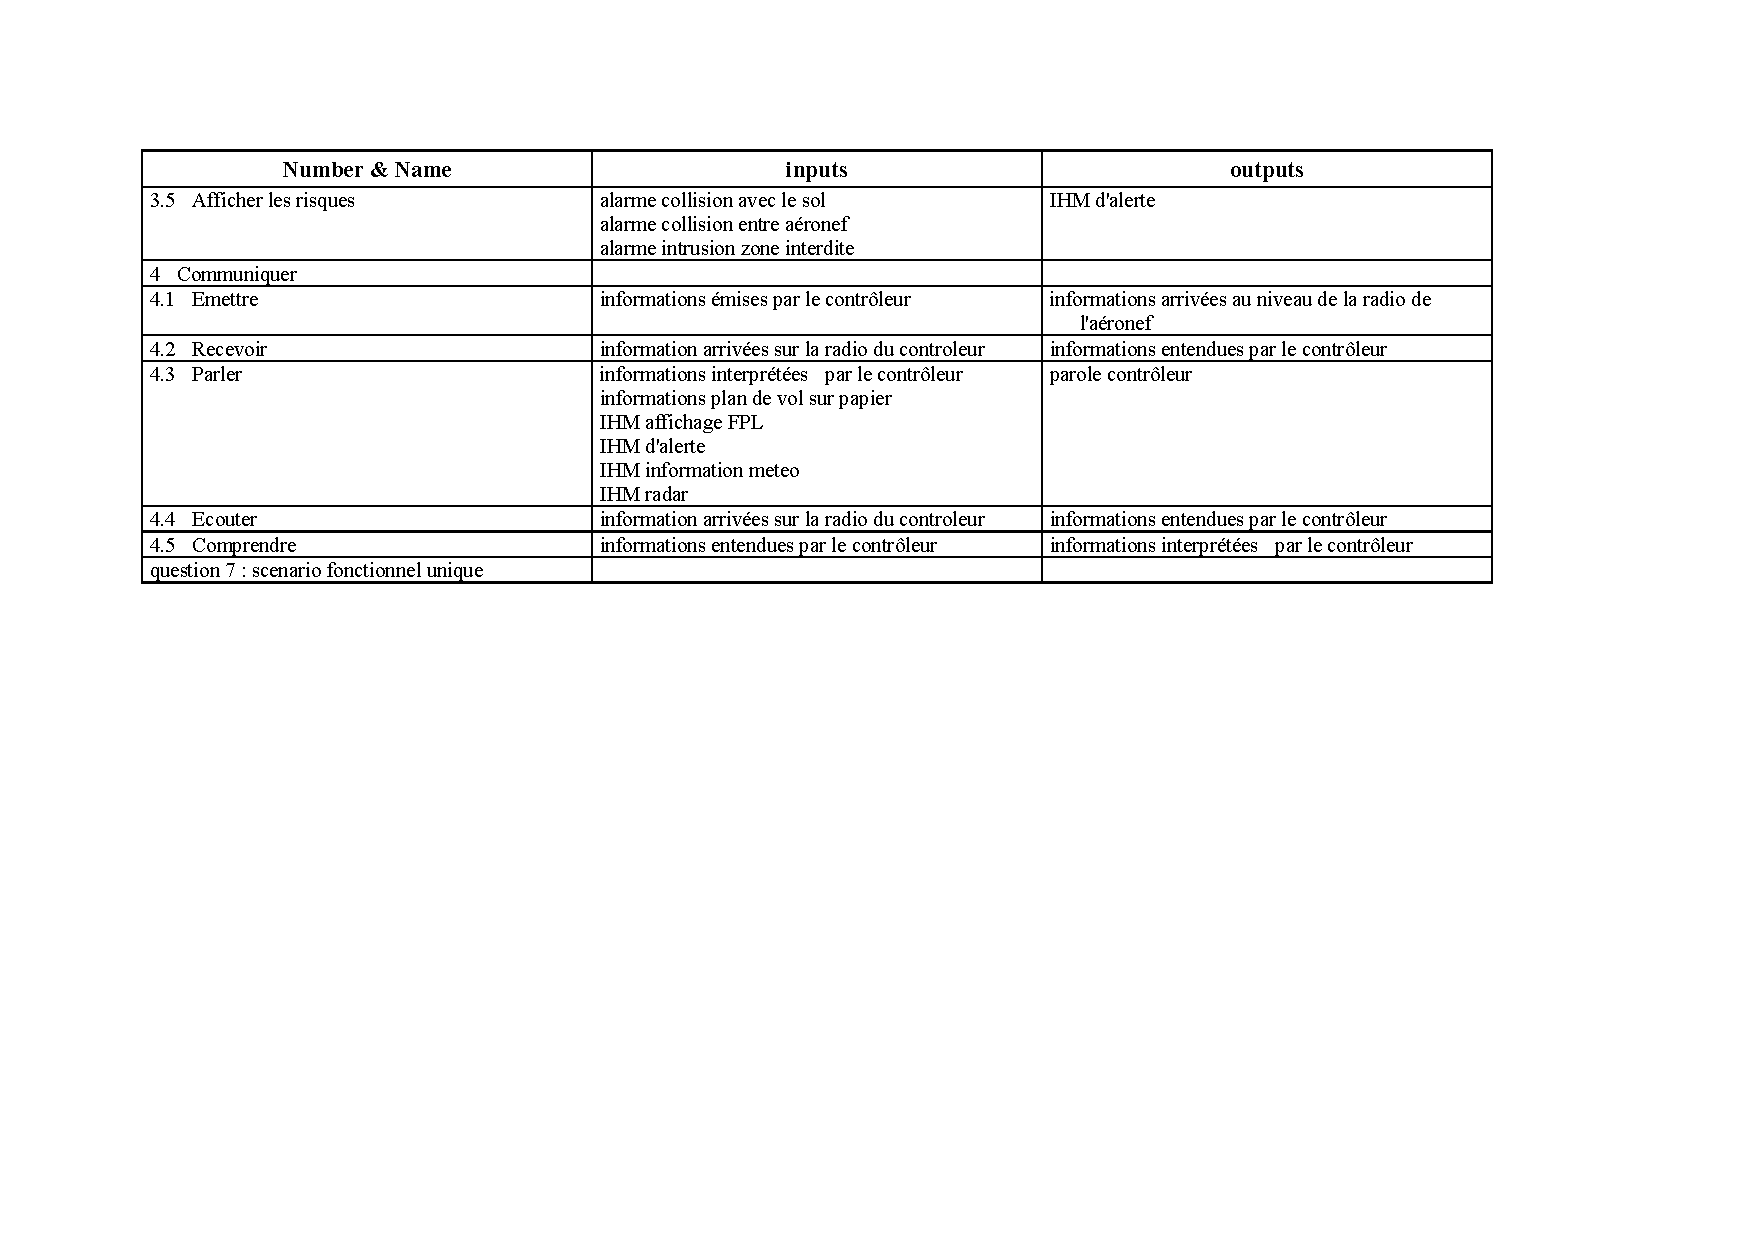
\includegraphics[scale=0.7]{images/tfio2}
			\caption{Matrice de traçabilité Fonctions / composants (suite)}
			\label{tfio2}
		\end{center}
	\end{figure}
	
\end{landscape}